\section{Results}
\label{sec:results}

This section covers what significance of the approach to collecting
runtime application I/O data using \Darshan. We present performance
analysis that shows how the new metrics helped provide more insight
results into I/O behavior and how this information can be represented
in Grafana.


Figure \ref{f:hacc} presents the mean number of I/O operations for
each HACC application and the error bar considering 95\% confidence
interval for the five jobs. This plot shows that even running at the
same system and with the same configuration, the applications
presented different I/O behavior. In fact, a single HPC application
can have multiple unique I/O behavior that can degradate the
performance of the application \cite{costa2021}. This I/O variation
can also happen between allocated devices. Figure \ref{f:hacc2} shows
the number of I/O requests per node for close and open operations for
two jobs for the HACC-IO application on Lustre for 10 millions
particles per rank.

\begin{figure}
	\centering
	% 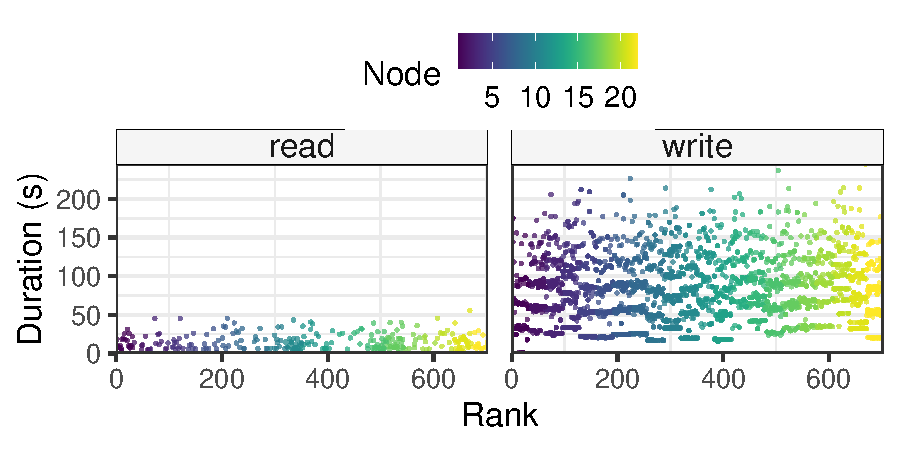
\includegraphics[width=\linewidth]{figs/255653_mpi_io_luster_no_coll_duration.pdf}
        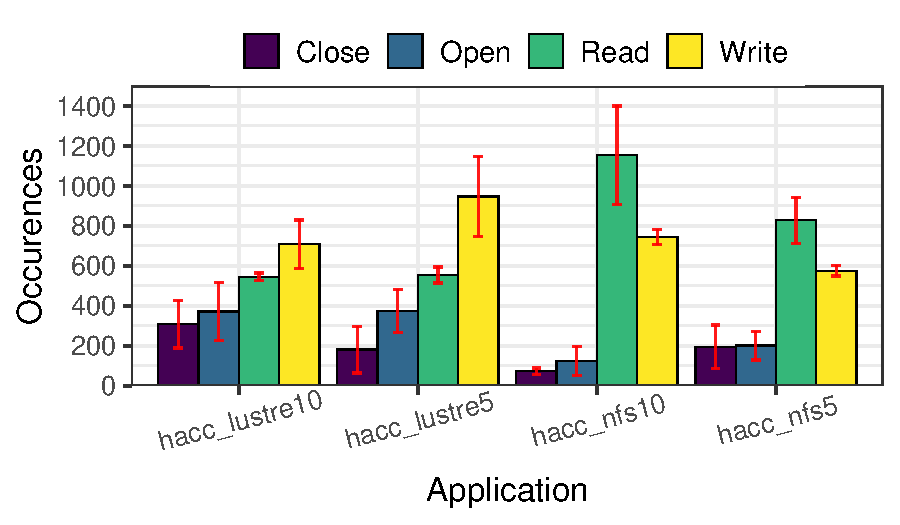
\includegraphics[width=\linewidth]{figs/operations_hacc.pdf}
	\caption{The same application can perform different amount of
          I/O operations during execution. It shows the mean
          occurences of each operation over the five job runs.}
	\label{f:hacc}
\end{figure}

% jobs "255515", "255675"
\begin{figure}
	\centering
        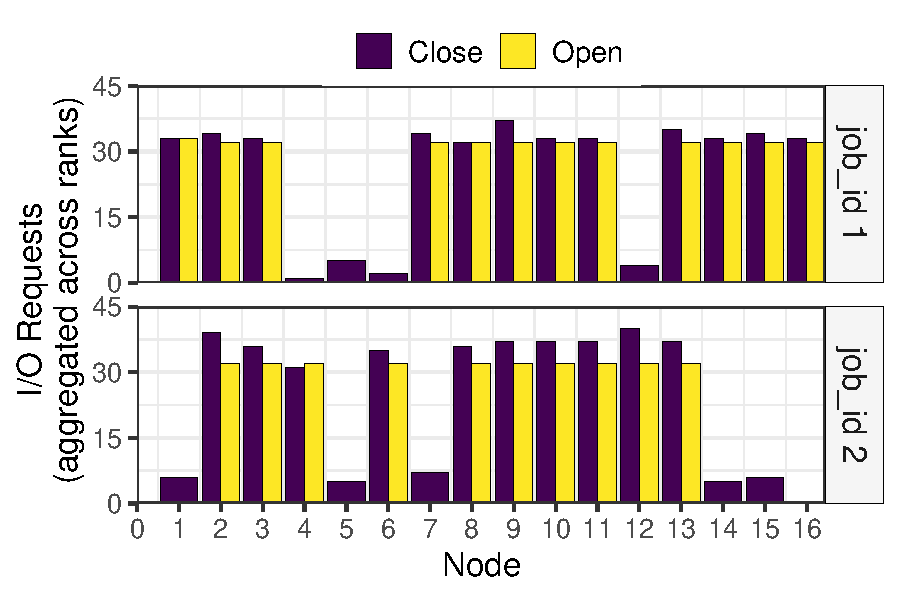
\includegraphics[width=\linewidth]{figs/hacc_nfs_10.pdf}
	\caption{The same application can perform different amount of
          I/O operations per node.}
	\label{f:hacc2}
\end{figure}

Figure \ref{f:mpi_io_all} shows the duration of the reads and writes
per rank for each execution (\texttt{job\_id} metric) of the MPI-IO
benchmark without using collective operations. We notice a similar
behavior for the I/O operations duration for all jobs except the
second one (\texttt{job\_id 2}). It presents a mean duration of 6.75
seconds for reads and 78s for writes, while the other jobs had a mean
duration of 0.05s for reads and 54s for writes. With the collected
logs, we can perform a spatial performance analysis to understand the
variability in the I/O behavior per system component, in this case,
per nodes and ranks.

\begin{figure}
	\centering
	% 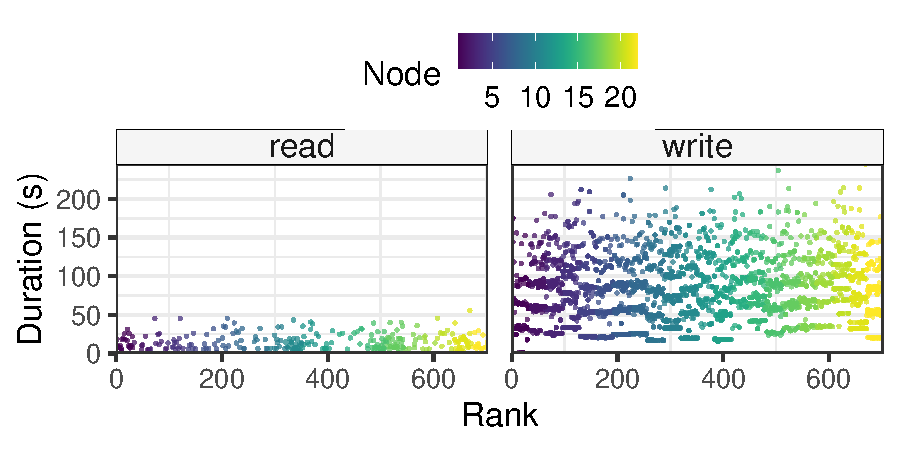
\includegraphics[width=\linewidth]{figs/255653_mpi_io_luster_no_coll_duration.pdf}
        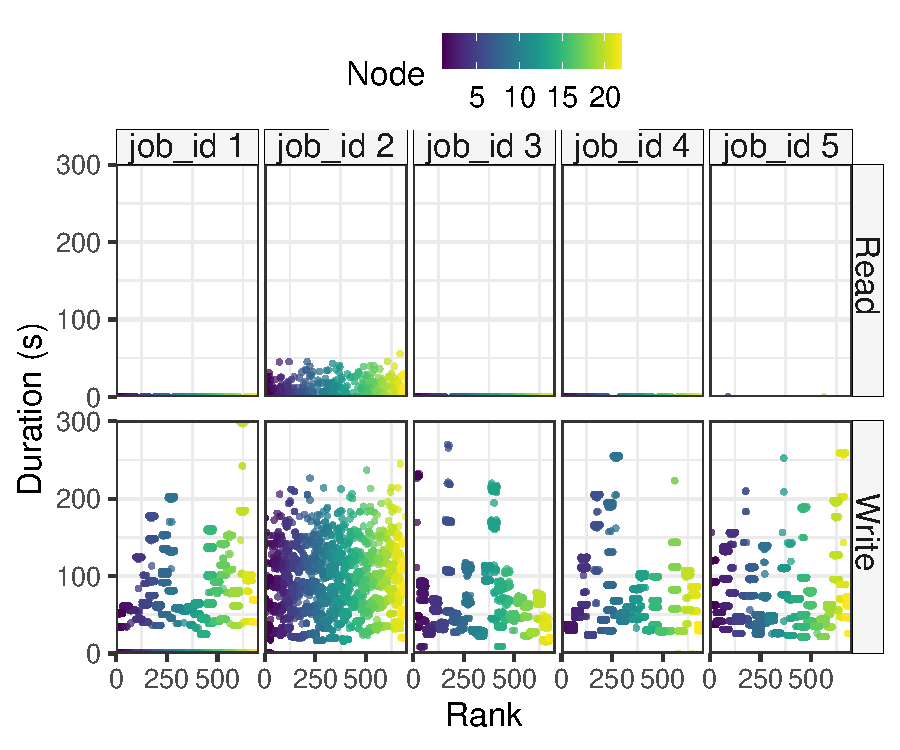
\includegraphics[width=\linewidth]{figs/mpi_io_luster_no_coll_duration_allexperiments.pdf}
	\caption{Jobs for the MPI-IO benchmark without collective
          operations presented variability in the number and duration
          of I/O operations.}
	\label{f:mpi_io_all}
\end{figure}

Using the absolute timestamps collected we can temporarily view
wherein the application execution the variability of a job
occured. Figure \ref{f:mpi_io} presents the duration and occurence of
I/O operations throughout the MPI-IO benchmark for \texttt{job\_id
  2}. We can identify the application I/O pattern of performing
writings during ten phases, and then reads at the end. Also, this
application run faster writes at the beginning and slower at the end,
with the slowest writting after 250 seconds.
      
\begin{figure}
	\centering
	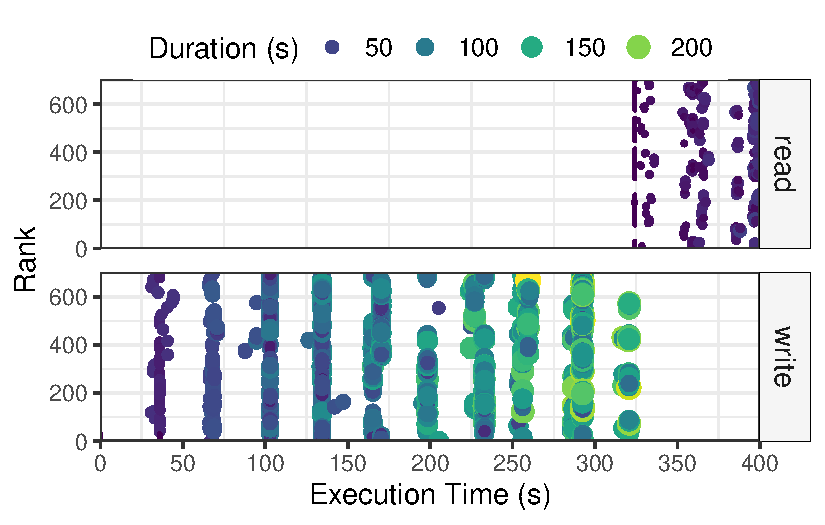
\includegraphics[width=\linewidth]{figs/255653_mpi_io_luster_no_coll_execution2.pdf}
	\caption{Distribution of reads and writes operations
          throughout the execution time for the \texttt{job\_id 2},
          can reveal the application I/O pattern, and wherein the
          application there were faster and slower operations.}
	\label{f:mpi_io}
\end{figure}

The same job is also represented in Figure \ref{f:mpi_io_grafana}
using the Grafana interface. This figure presents the number of I/O
writes (blues) and reads (green) and the amount of bytes sent
aggregated across ranks. The writes behavior shows the application
phases where it dealt with larger I/O sizes, with two moments writting
more than 20GB, while the reading operations run for a shorter moment
for aroun 12GB of I/O size. Grafana offers an interactive front-end
view where users can easily filter to visualize specific time and
metrics intervals. Such representation using the absolute timestamps
facilitates the correlation of I/O performance congestion, for
example, with system behavior monitoring, which can also be
represented as a Grafana dashboard.

\begin{figure*}[h!]
	\centering
	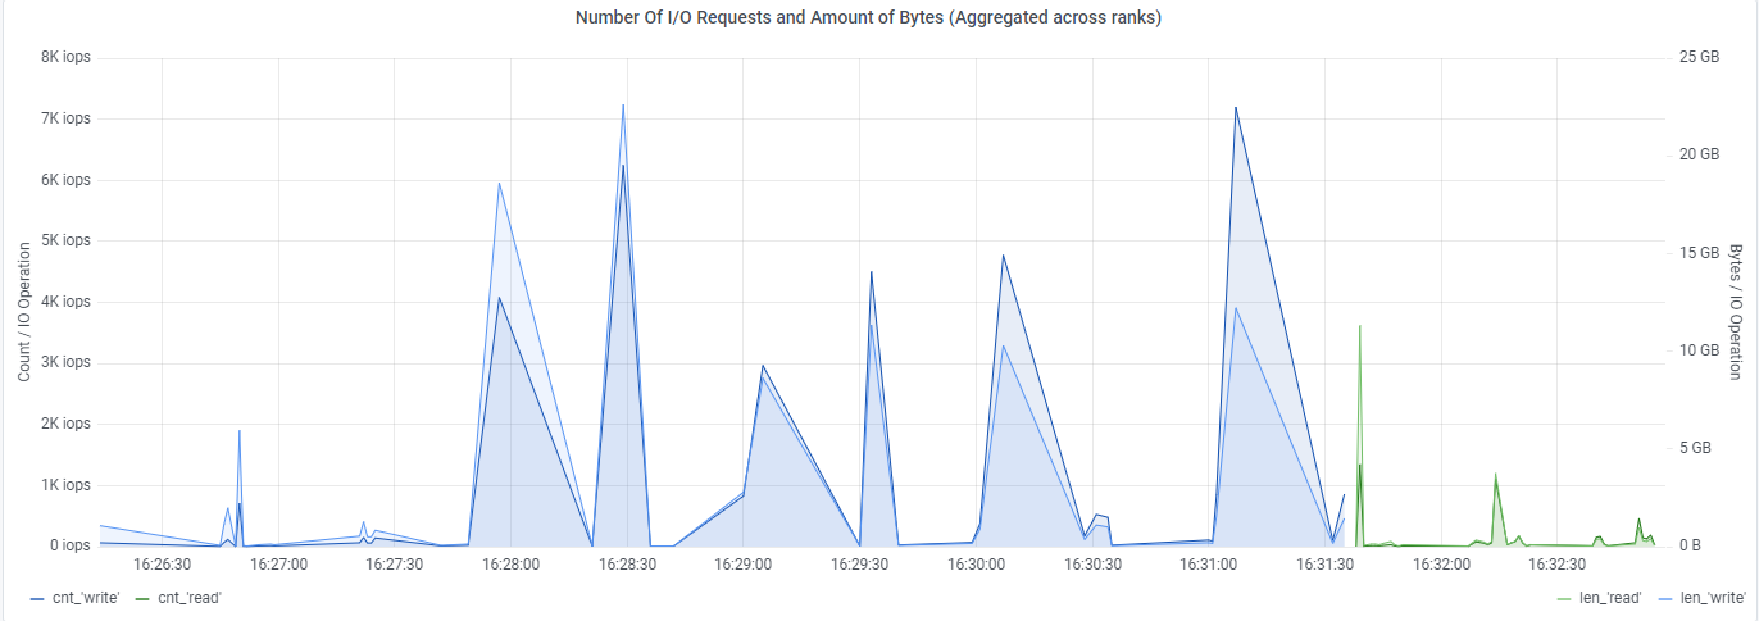
\includegraphics[width=\textwidth]{figs/255653_mpi_io_luster_no_coll.pdf}
	\caption{Graphana visualization of the \texttt{job\_id 2}
          writes and reads operations and amount of bytes per
          operation, using the absolute timestamp metric collected
          with \emph{Darshan LDMS Integration}.}
	\label{f:mpi_io_grafana}
      \end{figure*}
